\subsection{ALOCAÇÃO DE MATÉRIAS}

Durante os incrementos anterioriores, o otimizador gerava grades horárias que continham apenas os nomes dos professores alocados para aula. Em outras palavras, as grades eram matrizes nas quais as linhas eram os horários disponíveis, as colunas eram as salas e cada posição na matriz representava qual professor deveria ministrar a aula naquele horário.

A alocação dos professores é muito importante para a resolução do problema, pois apresenta a maior parte das retrições e dificuldades relacionadas, como os conflitos, por exemplo. Entretando, em termos de completude, as grades horárias devem ter também a alocação de matérias em cada horário de aula, visto que cada professor pode ministrar aulas de mais de uma matéria. As alterações necessárias para possibilitar isso foram:

\begin{enumerate}
	\item Alterar a modelagem do banco de dados para comportar informações relacionadas às matérias;
	\item Alterar telas da interface web para que fosse possível configurar as matérias;
	\item Alterar rotas do servidor para persistir as matérias;
	\item Alterar código do otimizador para produzir grades horárias com matérias
\end{enumerate}

\subsubsection{Alteração no banco de dados}
Para armazenar informações relacionadas às matérias, a modelagem do banco de dados foi alterada com a criação de três tabelas: 
\begin{itemize}
	\item materia
	\item horario-materias: representa uma grade horária de matérias, que tem vínculo com a entidade principal da grade horária
	\item horario-materia: representa uma matéria alocada em determinada posição de uma grade horária
\end{itemize}

Com esta modelagem atualizada, presente na figura \ref{fig:modelagemMateiras}, cada grade horária de professores, pode ter diferentes opções de grades de matérias.

\begin{figure}[!htb]
	\centering
	\caption{Modelo Entidade-Relacionamento com Matérias}
	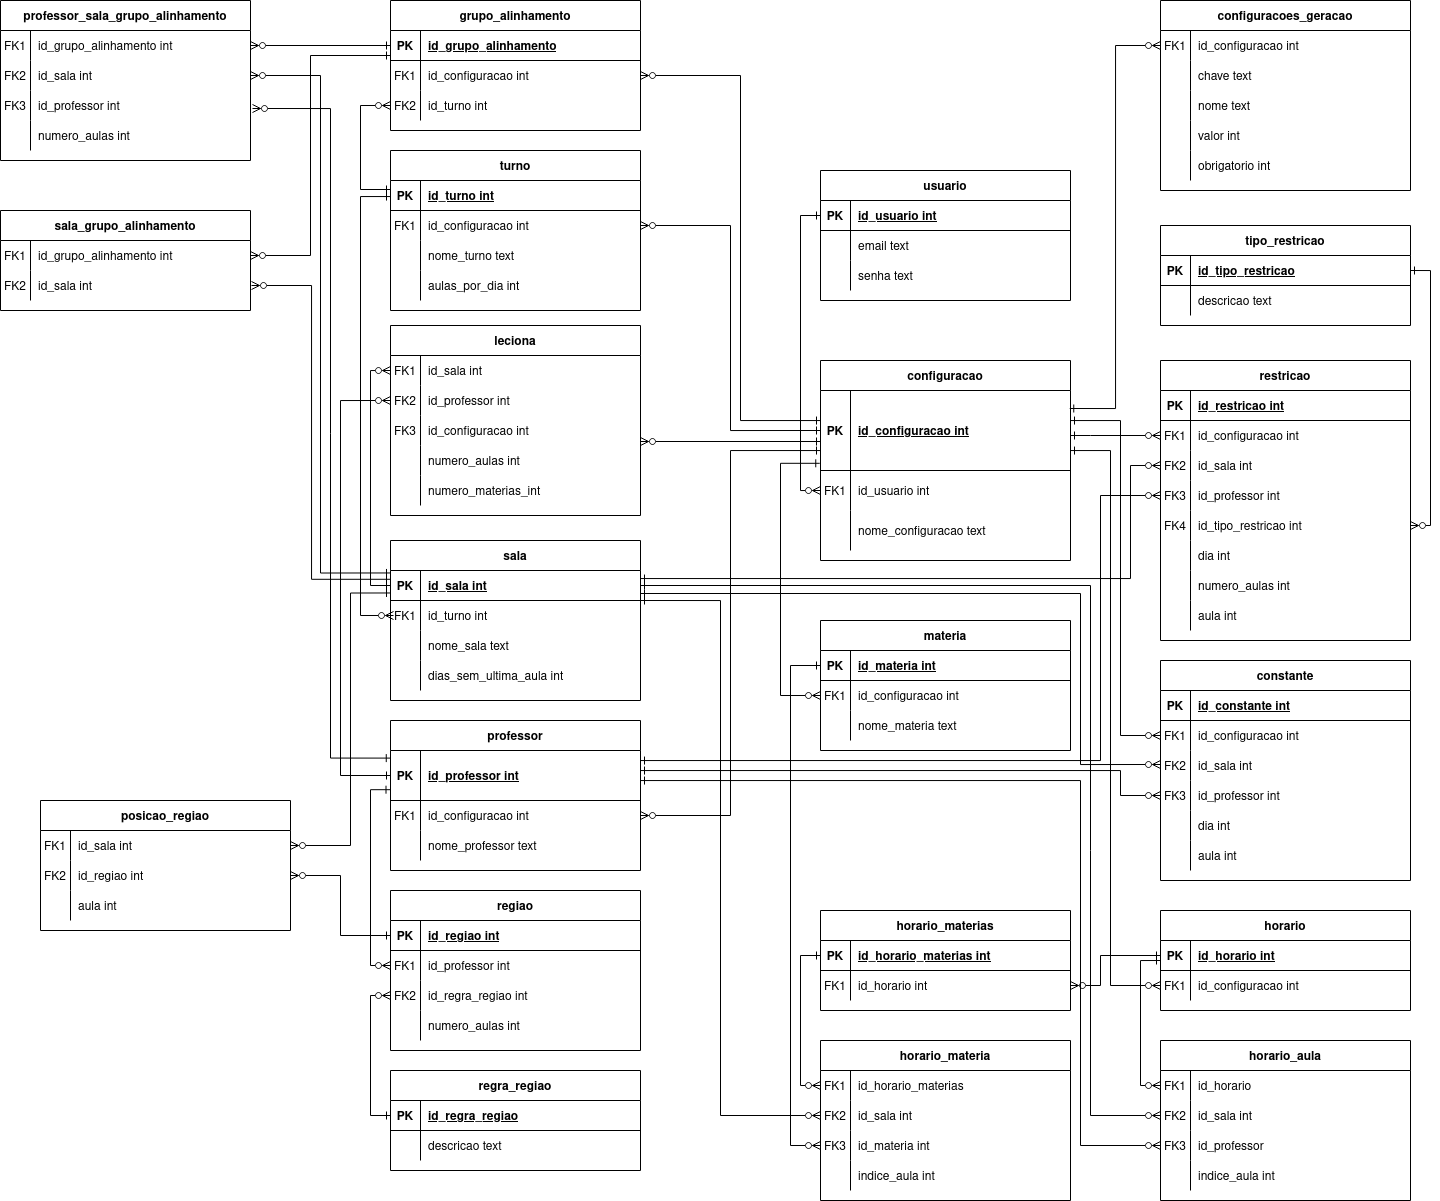
\includegraphics[width=0.65\textwidth]{./dados/figuras/er_materias}
	\fonte{Autor}
	\label{fig:modelagemMateiras}
\end{figure}
\pagebreak

\subsubsection{Alteração de telas}
Com a adição do conceito das matérias ao sistema, algumas telas da interface precisaram ser modificadas. A primeira destas, foi a tela inicial da configuração, ou seja, a tela de "Estrutura da Escola", cuja alteração pode ser vista na figura \ref{fig:estruturaAtualizada} consistiu na adição de uma seção para cadastro e visualização de matérias, semelhante ao componente de cadastro de professores.

\begin{figure}[!htb]
	\centering
	\caption{Estrutura da Escola com Matérias}
	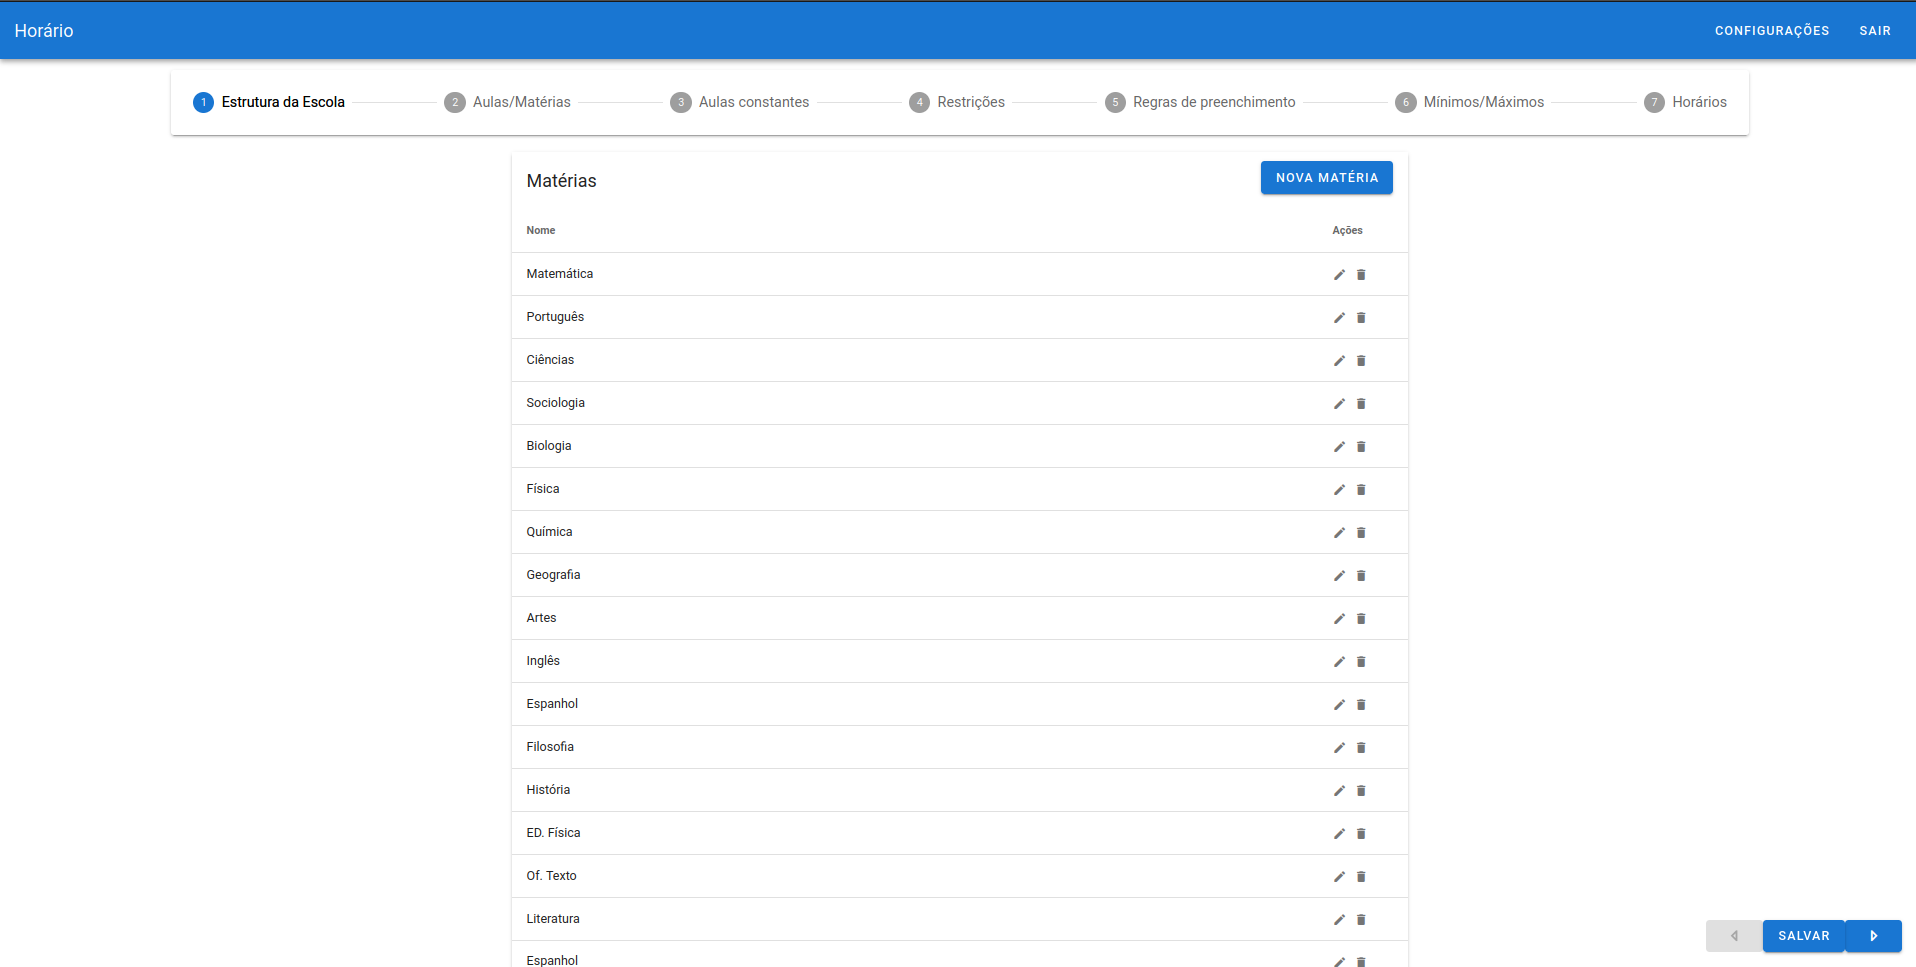
\includegraphics[width=0.65\textwidth]{./dados/figuras/alteracaoEstrutura}
	\fonte{Autor}
	\label{fig:estruturaAtualizada}
\end{figure}
\pagebreak

Além da tela de estrutura, a segunda aba da configuração ("Aulas/Matérias") foi alterada para que fosse possível vincular matérias aos professores, e configurar a quantidade de aulas de cada matéria deve ser ministrada semanalmente, conforme a figura \ref{fig:alteracaoAulas}.

\begin{figure}[!htb]
	\centering
	\caption{Tela de configuração de quantidades de aulas por matéria}
	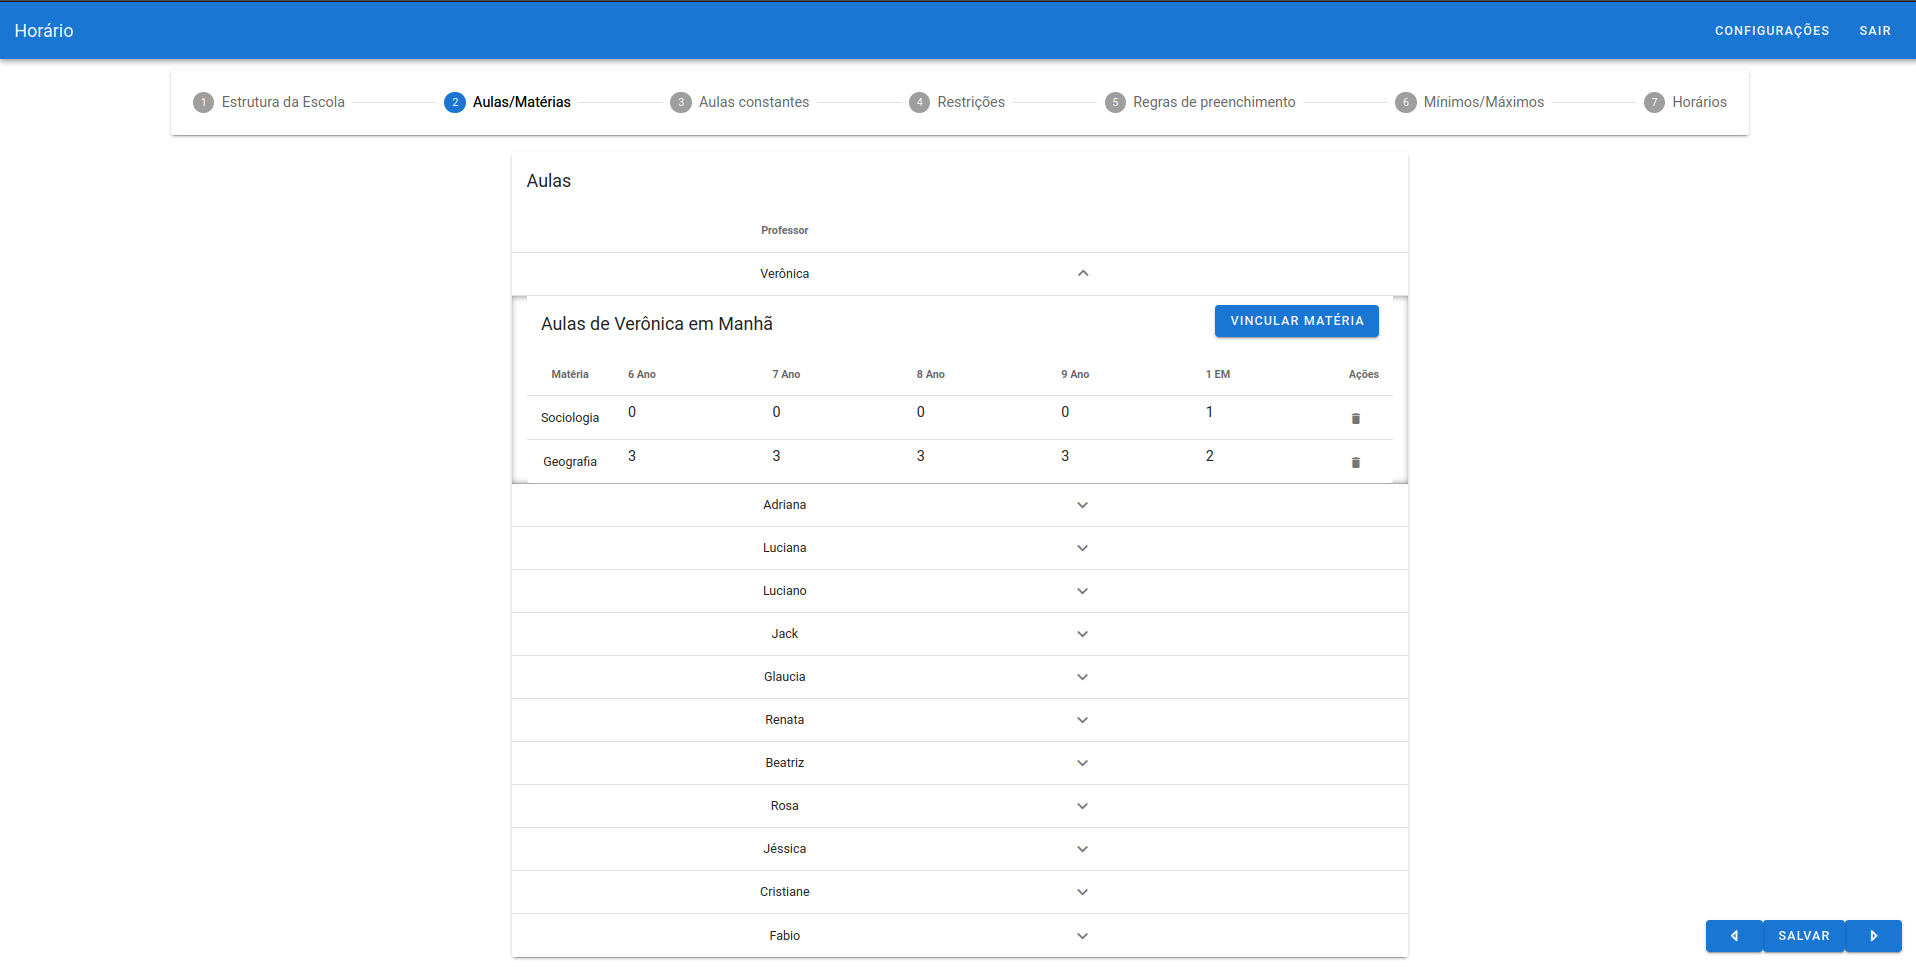
\includegraphics[width=0.65\textwidth]{./dados/figuras/alteracaoAulas}
	\fonte{Autor}
	\label{fig:alteracaoAulas}
\end{figure}

Por fim, na tela final da configuração, representável por exibir as grades horárias geradas, foi necessário alterar o componente da grade para incluir, além dos nomes dos professores, os nomes das matérias alocadas para cada horário, como pode ser visto na figura \ref{fig:alteracaoHorario}.

\begin{figure}[!htb]
	\centering
	\caption{Visualização de grade horária com matérias}
	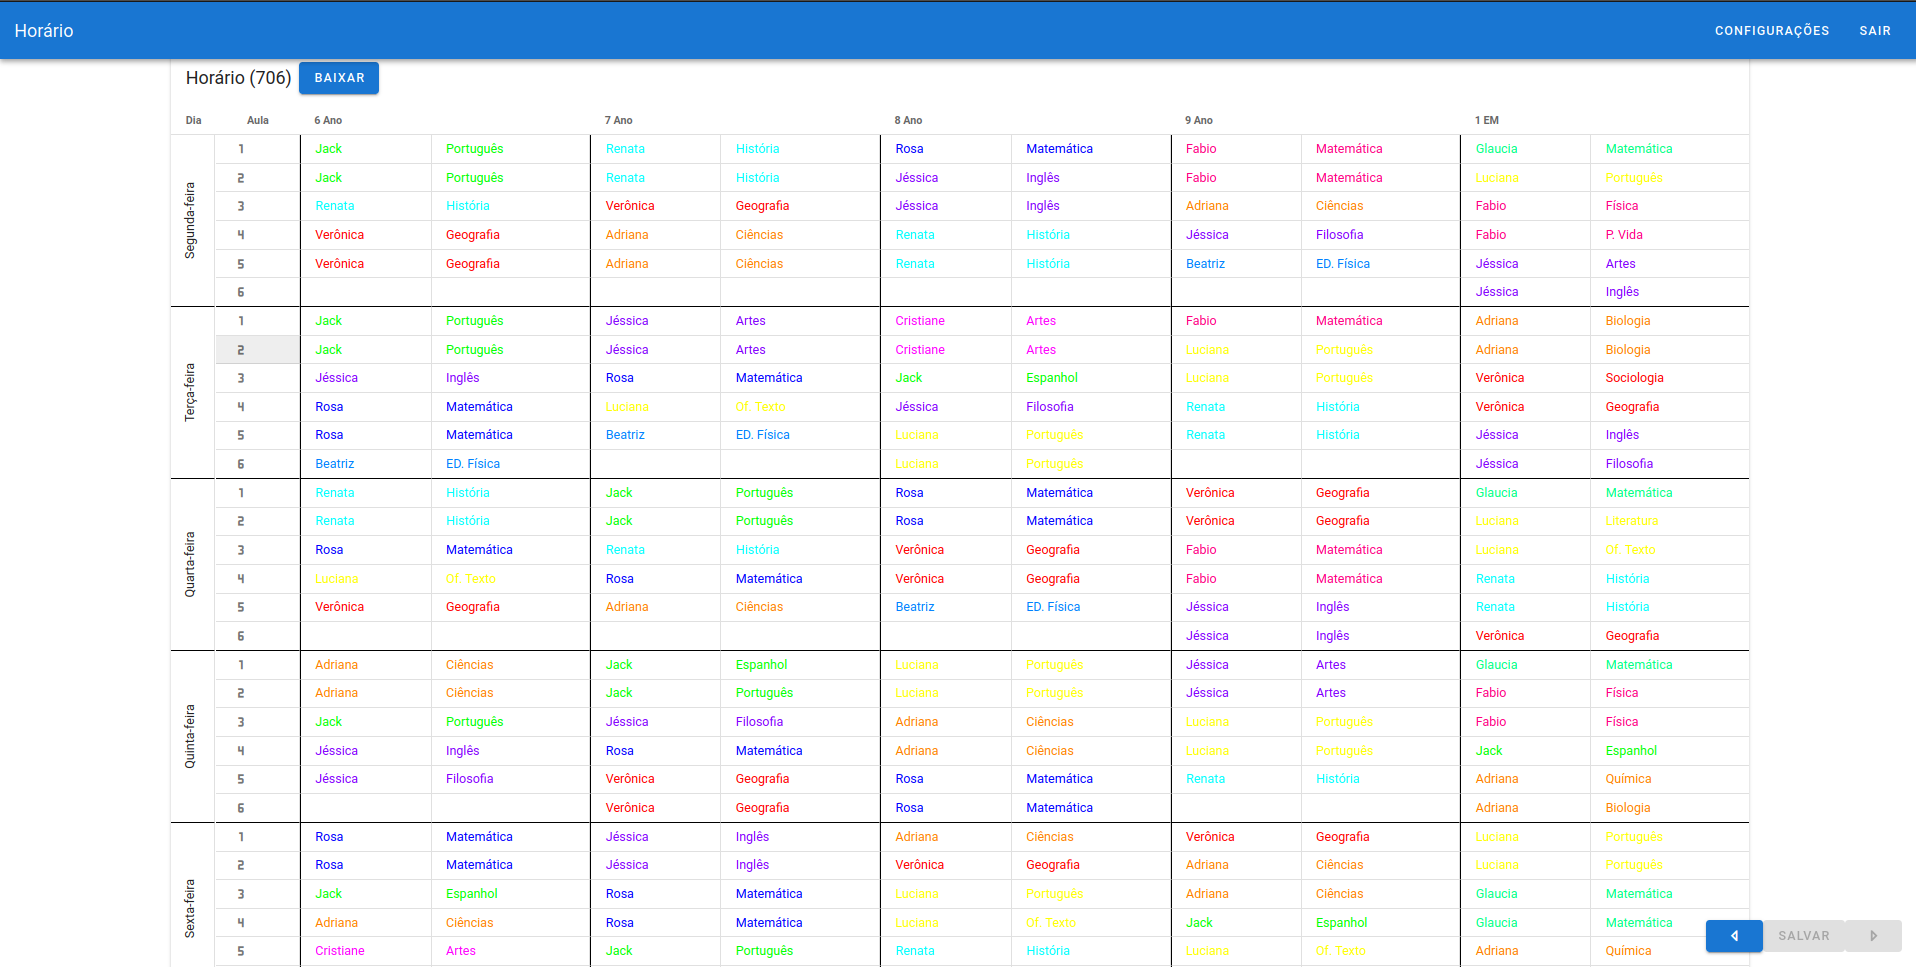
\includegraphics[width=0.65\textwidth]{./dados/figuras/alteracaoHorarios}
	\fonte{Autor}
	\label{fig:alteracaoHorario}
\end{figure}

\subsubsection{Alteração de métodos no servidor}
A adição das matérias também envolveu algumas alterações no servidor. As rotas alteradas para acomodar a melhoria foram rotas de armazenamento e consulta da estrutura da escola, aulas e grades horárias.

Evidentemente, as funções responsáveis por essas rotas precisaram ser modificadas para interagir corretamente com as novas tabelas criadas durante o desenvolvimento deste incremento.

\subsubsection{Matérias no otimizador}
Após as alterações na interface, servidor e banco de dados, o sistema estava pronto para lidar com as informações relacionadas às matérias, faltando apenas a incorporação destas na geração de grades horárias por parte do otimizador. Para realizar isso, implementou-se um método análogo ao \autoref{alg:otimizadorComRestricoes}, porém voltado à geração de grades de matérias.

A diferença é que o novo método implementado obtém determinada grade horária gerada pelo \autoref{alg:otimizadorComRestricoes}, e realiza as operações necessárias para preencher a grade com matérias. Vale ressaltar que essas operações são semelhantes à geração da grade de aulas dos professores: preenchimento da grade inicial, cálculo da variação de custo, realização de trocas de posições e armazenamento das soluções.

O método de geração de grades foi aplicado no otimizador de forma que cada vez que uma grade horária de professores é salva no banco de dados, esta também já tem a sua grade horária de matérias gerada, completando assim o processo de otimização da grade, conforme o \autoref{alg:otimizadorCompleto}.

\begin{algorithm}
	\caption{Otimizador com matérias}
	\label{alg:otimizadorCompleto}
	\KwIn{Lista de professores $LP$, lista de turmas $LT$, matriz de aulas e matérias por professor por turma $MA$, temperatura inicial $TI$, Taxa de resfriamento $TR$}
	\KwOut{Grade horária de matérias e professores otimizada}
	$temperatura \leftarrow TI$\\
	$grade \leftarrow$ CriaGradeInicial$(LP, LT, MA)$\\
	$iteracoesSemAlteracao \leftarrow 0$\\
	$solucoes \leftarrow$ lista vazia\\
	\While {condição de parada não atingida} {
		$deltaTotal \leftarrow 0$\\
		\For {$passo = 0$ até $numeroPassos$} {
			$turma \leftarrow grade.EscolheTurmaAleatoria()$\\
			$linhas \leftarrow grade.EscolheHorariosAleatoriosValidos(sala)$\\
			$delta \leftarrow grade.CalculaDelta(sala, linhas)$\\
			$probabilidade \leftarrow e^{-delta/temperatura}$\\
			$valorAceite \leftarrow Aleatorio(0, 1)$\\
			\If {$delta < 0$ ou $probabilidade \ge valorAceite$} {
				$grade.PermutaProfessores(sala, linha1, linha2)$\\
				$deltaTotal \leftarrow deltaTotal + delta$\\
				\If {grade não existe na lista de soluções} {
					insere grade na lista de soluções\\
					limita lista de soluções às 100 melhores grades\\
				}
			}
		}
		\eIf {$delta = 0$} {
			$iteracoesSemAlteracao \leftarrow iteracoesSemAlteracao + 1$\\
		}{
			$iteracoesSemAlteracao \leftarrow 0$\\
		}
		\If {$iteracoesSemAlteracao \ge 15$} {
			\For{gradeProfessores em EscolherGradesRelevantes(solucoes)} {
				SalvaGradeProfessores$(gradeProfessores)$\\
				$gradesMaterias \leftarrow$ GeraGradesMaterias$(gradeProfessores)$\\
				SalvarMelhorGradeMaterias$(gradesMaterias)$\\
			}
			apaga lista de soluções\\
			$temperatura \leftarrow TI$\\
			$iteracoesSemAlteracao \leftarrow 0$\\
		}
		$temperatura \leftarrow temperatura * TR$
	}
\end{algorithm}
